% How to Draw Flowcharts in LaTeX using TikZ?
% latexdraw.com
% 30/01/2021 at 00:07

\documentclass[border=0.2cm]{standalone}

% Required packages
\usepackage{tikz}
\usetikzlibrary{shapes,positioning}

\begin{document}

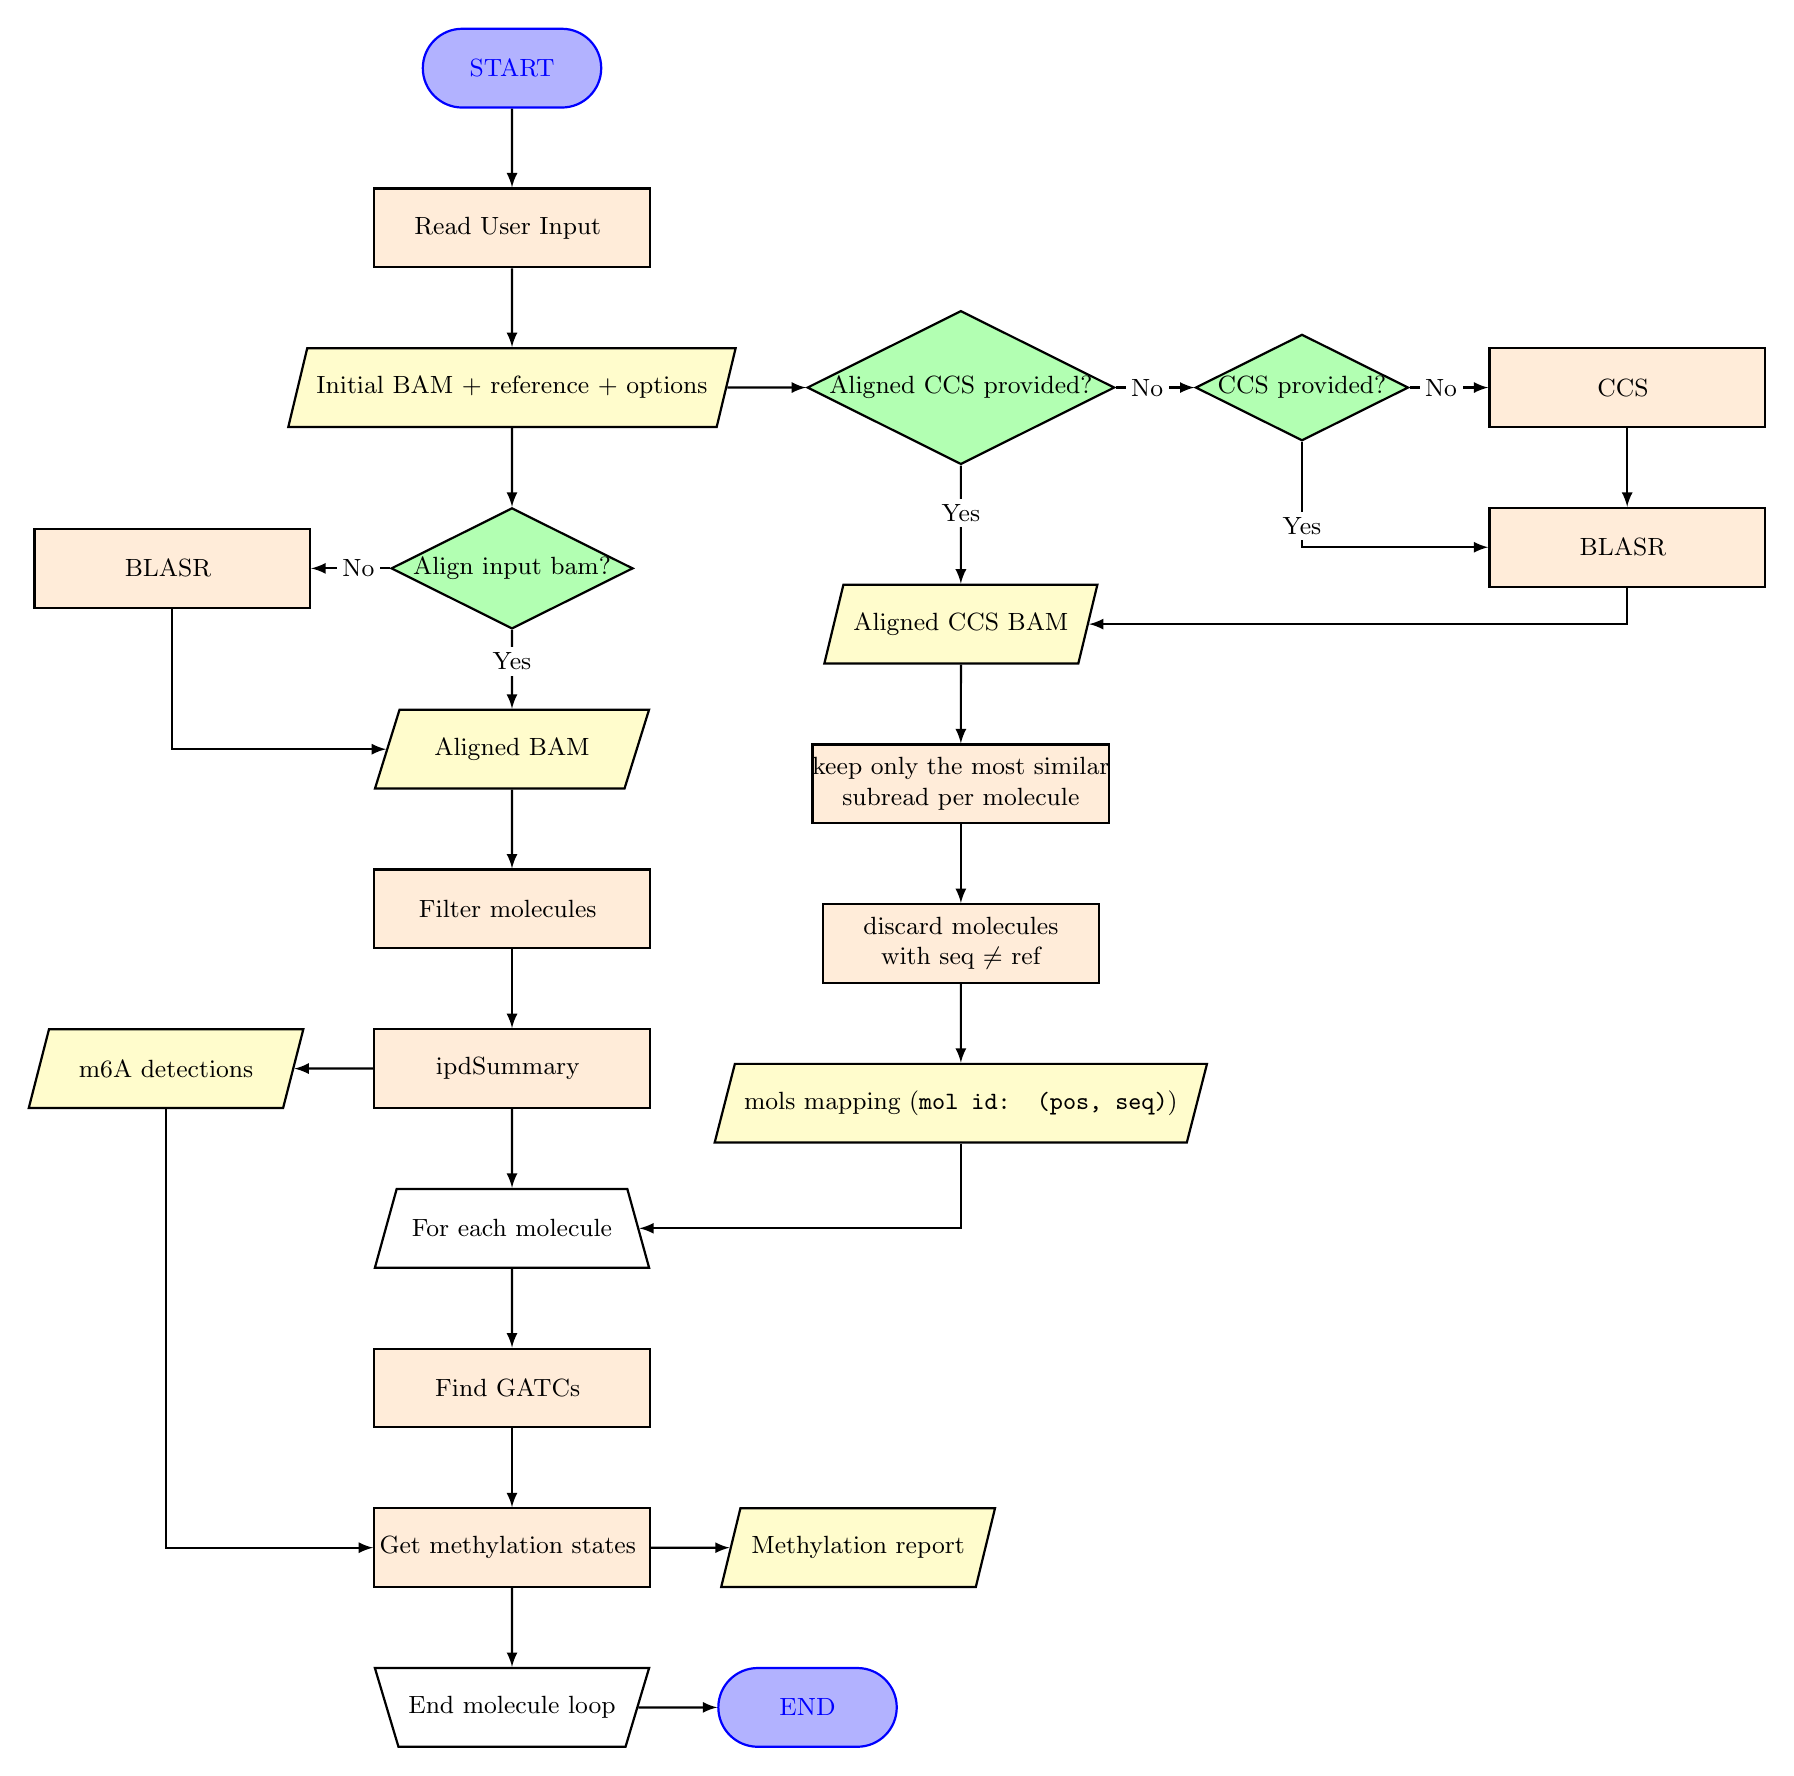
\begin{tikzpicture}[font=\small,thick]

% Start block
\node[draw, blue,
    rounded rectangle,
    minimum width=2.5cm,
    fill=blue!30,
    minimum height=1cm] (start) {START};


\node[draw, 
    align=center,
    below=of start,
    fill=orange!15,
    minimum width=3.5cm,
    minimum height=1cm
] (input) { Read User Input };

\node[draw,
    trapezium, 
    trapezium left angle = 65,
    trapezium right angle = 115,
    trapezium stretches,
    fill=yellow!20,
    below=of input,
    minimum width=3.5cm,
    minimum height=1cm
] (inputparameters) { Initial BAM + reference + options };

% Conditions test
\node[draw,
  diamond,
  fill=green!30,
    right=of inputparameters,
    aspect=2,
    minimum width=2.5cm,
    inner sep=0] (alignedccsgiven) { Aligned CCS provided? };

\node[draw,
  diamond,
  fill=green!30,
  %xshift=1cm,
    right=of alignedccsgiven,
    aspect=2,
    minimum width=2.5cm,
    inner sep=0] (ccsgiven) { CCS provided? };

\node[draw,
    align=center,
    right=of ccsgiven,
    fill=orange!15,
    minimum width=3.5cm,
    minimum height=1cm,
    inner sep=0] (ccs) { CCS };

\node[draw,
    align=center,
    below=of ccs,
    fill=orange!15,
    minimum width=3.5cm,
    minimum height=1cm,
    inner sep=0] (alignccs) { BLASR };

\node[draw,
    trapezium, 
    trapezium left angle = 65,
    trapezium right angle = 115,
    trapezium stretches,
    fill=yellow!20,
    below=of alignedccsgiven,
    minimum width=3.5cm,
    minimum height=1cm,
    yshift=-5mm
] (alignedccs) { Aligned CCS BAM };

\node[draw,
    align=center,
    below=of alignedccs,
    fill=orange!15,
    minimum width=3.5cm,
    minimum height=1cm,
    inner sep=0] (filtersimilarityratio) { keep only the most similar\\subread per molecule };

\node[draw,
    align=center,
    below=of filtersimilarityratio,
    fill=orange!15,
    minimum width=3.5cm,
    minimum height=1cm,
    inner sep=0] (filterseqs) { discard molecules\\with seq $\neq$ ref };

\node[draw,
    trapezium, 
    trapezium left angle = 65,
    trapezium right angle = 115,
    trapezium stretches,
    fill=yellow!20,
    below=of filterseqs,
    minimum width=3.5cm,
    minimum height=1cm
] (molsmapping) { mols mapping (\texttt{mol id: (pos, seq)}) };

\node[draw,
  diamond,
  fill=green!30,
    below=of inputparameters,
    aspect=2,
    minimum width=2.5cm,
    inner sep=0] (alignedbamgiven) { Align input bam? };

\node[draw,
    trapezium, 
    trapezium left angle = 65,
    trapezium right angle = 115,
    trapezium stretches,
    fill=yellow!20,
    below=of alignedbamgiven,
    minimum width=3.5cm,
    minimum height=1cm
] (alignedbam) { Aligned BAM };

\node[draw,
    align=center,
    left=of alignedbamgiven,
    fill=orange!15,
    minimum width=3.5cm,
    minimum height=1cm,
    inner sep=0] (alignbam) { BLASR };

\node[draw,
    align=center,
    below=of alignedbam,
    fill=orange!15,
    minimum width=3.5cm,
    minimum height=1cm,
    inner sep=0] (filtermols) { Filter molecules };

\node[draw,
    align=center,
    below=of filtermols,
    fill=orange!15,
    minimum width=3.5cm,
    minimum height=1cm,
    inner sep=0] (ipdSummary) { ipdSummary };

\node[draw,
    trapezium, 
    trapezium left angle = 65,
    trapezium right angle = 115,
    trapezium stretches,
    fill=yellow!20,
    left=of ipdSummary,
    minimum width=3.5cm,
    minimum height=1cm
] (detections) { m6A detections };

\node[draw,
    trapezium, 
    trapezium stretches,
    below=of ipdSummary,
    minimum width=3.5cm,
    minimum height=1cm
] (formol) { For each molecule };

\node[draw,
    align=center,
    below=of formol,
    fill=orange!15,
    minimum width=3.5cm,
    minimum height=1cm,
    inner sep=0] (findgatcs) { Find GATCs };

\node[draw,
    align=center,
    below=of findgatcs,
    fill=orange!15,
    minimum width=3.5cm,
    minimum height=1cm,
    inner sep=0] (getmethstates) { Get methylation states };

\node[draw,
    trapezium, 
    trapezium left angle = 120,
    trapezium right angle = 120,
    trapezium stretches,
    below=of getmethstates,
    minimum width=3.5cm,
    minimum height=1cm
] (endformol) { End molecule loop };

\node[draw,
    trapezium, 
    trapezium left angle = 65,
    trapezium right angle = 115,
    trapezium stretches,
    fill=yellow!20,
    right=of getmethstates,
    minimum width=3.5cm,
    minimum height=1cm
] (methreport) { Methylation report };

\node[draw, blue,
  rounded rectangle,
  fill=blue!30,
    right=of endformol,
    minimum width=2.5cm,
    minimum height=1cm] (end) {END};


\draw[-latex] (start) edge (input)
    (input) edge (inputparameters)
    (inputparameters) edge (alignedccsgiven)
    (inputparameters) edge (alignedbamgiven)
    (ccs) edge (alignccs)
    (alignedccs) edge (filtersimilarityratio)
    (filtersimilarityratio) edge (filterseqs)
    (filterseqs) edge (molsmapping)
    (alignedbam) edge (filtermols)
    (filtermols) edge (ipdSummary)
    (ipdSummary) edge (detections)
(ipdSummary) edge (formol)
(formol) edge (findgatcs)
(findgatcs) edge (getmethstates)
(getmethstates) edge (methreport)
(getmethstates) edge (endformol)
(endformol) edge (end);

\draw[-latex] (alignedccsgiven) edge node[pos=0.4,fill=white,inner sep=2pt]{Yes}(alignedccs)
    (alignedccsgiven) edge node[pos=0.4,fill=white,inner sep=2pt]{No}(ccsgiven.west);

\draw[-latex] (ccsgiven) edge node[pos=0.4,fill=white,inner sep=2pt]{No}(ccs.west)
    (ccsgiven) |- (alignccs) node[pos=0.4,fill=white,inner sep=2pt]{Yes};

\draw[-latex] (alignccs) |- (alignedccs);

\draw[-latex] (alignedbamgiven) edge node[pos=0.4,fill=white,inner sep=2pt]{No}(alignbam)
    (alignedbamgiven) edge node[pos=0.4,fill=white,inner sep=2pt]{Yes}(alignedbam);

\draw[-latex] (alignbam) |- (alignedbam);

\draw[-latex] (molsmapping) |- (formol);

\draw[-latex] (detections) |- (getmethstates);
\end{tikzpicture}

\end{document}
